
%(BEGIN_QUESTION)
% Copyright 2006, Tony R. Kuphaldt, released under the Creative Commons Attribution License (v 1.0)
% This means you may do almost anything with this work of mine, so long as you give me proper credit

Graph {\it just the derivative response} a proportional+derivative controller to the following input conditions, assuming a proportional band of 500\% and a derivative constant of 1.5 minutes.  The controller's action is {\it direct}, and the algorithm it follows is shown below the graph:

$$\includegraphics[width=15.5cm]{i01547x01.eps}$$

The time scale on the chart is minutes:seconds, and the P+D algorithm is as follows:

$$m = K_p \left( e + \tau_d {de \over dt} \right) + b$$

\noindent
Where,

$m$ = Controller output (manipulated variable)

$K_p$ = Gain

$e$ = Error signal (PV$-$SP)

$\tau_d$ = Derivative time constant

$b$ = Bias

\vskip 10pt

\underbar{file i01547}
%(END_QUESTION)





%(BEGIN_ANSWER)

$$\includegraphics[width=15.5cm]{i01547x02.eps}$$

First, let us understand that a proportional band of 500\% is equivalent to a gain of 1/5, or 0.2.

\vskip 10pt

The downward step-change of the PV at time 0:30 causes the derivative to saturate the output to 0\%.  When the PV levels off, the derivative response goes to 0, leaving the output at the value where it started (60\%).

From 1:00 to 1:30, the PV ramps from 15\% to 35\%, for a de/dt slope of +40\% per minute.  Multiplied by a $\tau_d$ constant of 1.5 and a gain ($K_p$) of 0.2, the derivative term's contribution is +12\%.  Thus, the output steps from 60\% to 72\%.

At 1:30, the PV ramp increases to a rate of 100\% per minute (from 35\% to 60\% over 15 seconds), resulting in a derivative term output of +30\%.  Thus, the output steps to new level of 90\% (original 60\% value + 30\% = 90\%).

Between 1:45 and 2:15 the PV slopes negatively.  This results in a negative derivative response (60\% to 35\% over 30 seconds = -50\% per minute, times 1.5 times 0.2 = -15\%).  Thus, the output goes from 60\% to 45\%.

At 2:15, the PV levels off and the derivative response ceases, leaving the output at its original value of 60\%

%(END_ANSWER)





%(BEGIN_NOTES)

 
%INDEX% Control, proportional + derivative: graphing controller response

%(END_NOTES)


